\section{Experimental Results}\label{sec:exp}
%
In this section, we present our experimental setup and the impact of the different optimizations and implementations described in the previous section. \\
%
\mypar{General note about the presented plots}
In all the plots that are presented in this section the marker symbol locates the mean of each measurement while the variance of the data is shown as a probability density around that mean value.
For the computation of the speedup on $n$ threads defined as $t_1/t_n$ the mean value of the one-threaded timing $t_1$ of the parallel code was used.
All time measurements were performed using the C++ high precision clock and a list of these single-threaded timings can be found in table \ref{tab:t1timings} (the 95\% confidence interval of each set of measurements of $t_1$ is less than $\pm 10\%$ around the mean). \\
\par\medskip
{\Large TODO: timing table}
\par\medskip
The discussion in this paper will focus on the topological sorting of a random graph with average node degree 32 and a base size of 1Mio nodes.\footnote{All plots in this section refer to graphs with 1Mio nodes except for the weak scaling graphs where the base size is 1Mio and the effective size in each execution is given by number~of~threads~$\times$~1Mio} 
While the speedup of our algorithms highly depend on the graph type (and in particular on its density), the relative positioning of different optimization strategies is consistent between all the graphs that were tested. \\
For a more comprehensive overview with more detailed scaling plots we refer to the project's Git repository (see link below).

%%%%%%%%%%%%%%%%%%%%%%%%%%%%%%%%%%%%%%%%%%%%%%%%%%%%%%%%%%%%%%%%%
% HARDWARE AND COMPILER
%%%%%%%%%%%%%%%%%%%%%%%%%%%%%%%%%%%%%%%%%%%%%%%%%%%%%%%%%%%%%%%%%
\mypar{Hardware and compiler}
  \begin{table}[h]
    \centering
    \begin{tabular}{ll}
    \toprule
    Processor        & Intel Xeon E5-2697 (Ivy bridge) \\
    Max. clock rate  & 3.5 GHz (with TurboBoost)\\
    \# Sockets       & 2 \\
    Cores / socket   & 12 \\
    Threads / socket & 24 \\
    LLC / socket     & 30 MB \\
    \midrule
    Compiler and flags & GCC 4.8.2, -O3\\
    \bottomrule
    \end{tabular}
    \caption{Hardware and compiler used for benchmarks}
    \label{tab:hardware}
  \end{table}
 
The following experiments were run on a 24-core system consisting of 2 Intel Xeon E5 processors (see table \ref{tab:hardware}).
Hyperthreading was not used for the benchmarks.
The implementations were written in \Cpp, using OpenMP and GCC atomic built-in functions. The graph was stored in an adjacency list.



\mypar{Effect of Optimization Strategies}
How does the initial, naive code compare to code that was enhanced with the Node-Lookup, Worksteal and other optimizations?
Figure \ref{fig:abstiming} shows the absolute timing of all the different algorithms that were implemented in this project.
\par\medskip
{\Large TODO: discussion}
\par\medskip
%
\begin{figure}[ht]
	\centering
	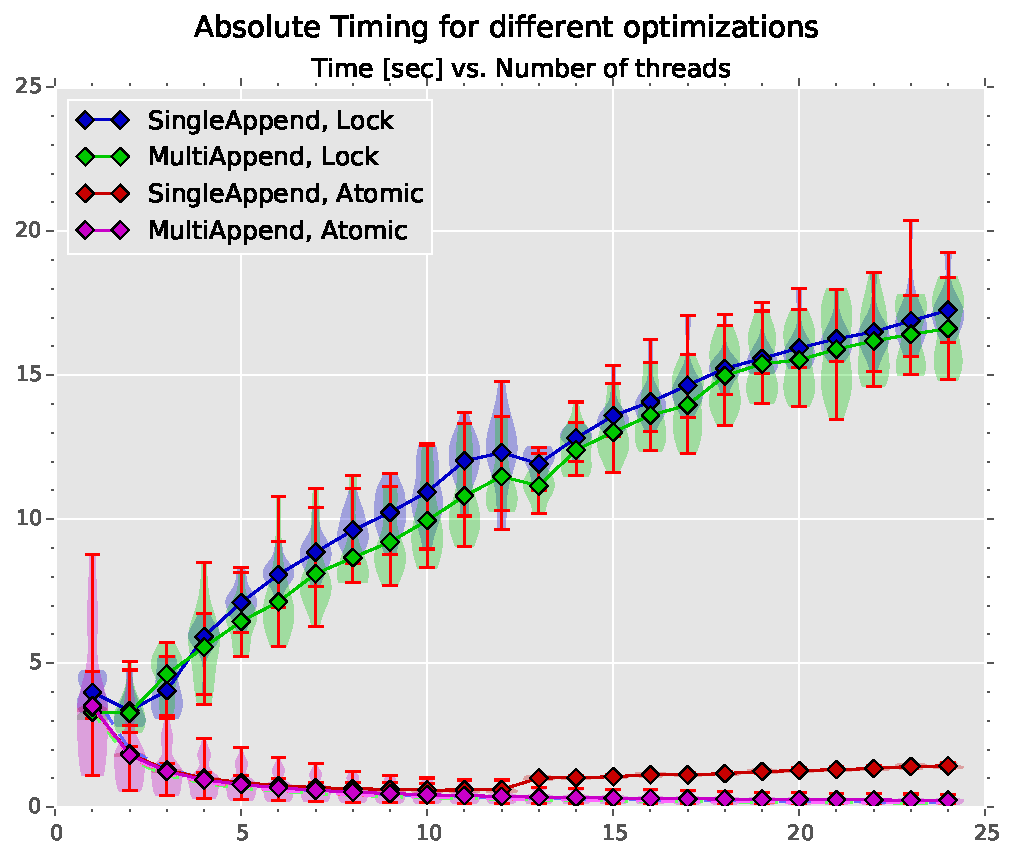
\includegraphics[width=\columnwidth]{plots/abstiming_gtRANDOMLIN_n1000000_deg30.pdf}
	\caption{To compare the effect of different optimizations, the Node-Lookup implementation was benchmarked with the respective optimizations turned on or off.
	As input graph, the random graph with node degree 30 was used.}
	\label{fig:abstiming}
\end{figure}

%%%%%%%%%%%%%%%%%%%%%%%%%%%%%%%%%%%%%%%%%%%%%%%%%%%%%%%%%%%%%%
% BENCHMARKS
%%%%%%%%%%%%%%%%%%%%%%%%%%%%%%%%%%%%%%%%%%%%%%%%%%%%%%%%%%%%%%

\mypar{Benchmarks of Optimization Strategies}
So far we have seen that the Node-Lookup and Worksteal algorithms do in fact allow us to speed up the topological sorting by using multiple threads.
Next we want to look at the scaling behavior of the optimized algorithms to see which ones perform better. \\
The weak and strong scaling plots are shown in figure \ref{fig:weakscaling} and \ref{fig:strongscaling} respectively.
Both plots confirm a relatively good scaling of both the Workstealing and the Node-Lookup techniques, with the Node-Lookup showing better absolute timing and better scaling in both cases. \\
%
\begin{figure}[ht]
	\centering
	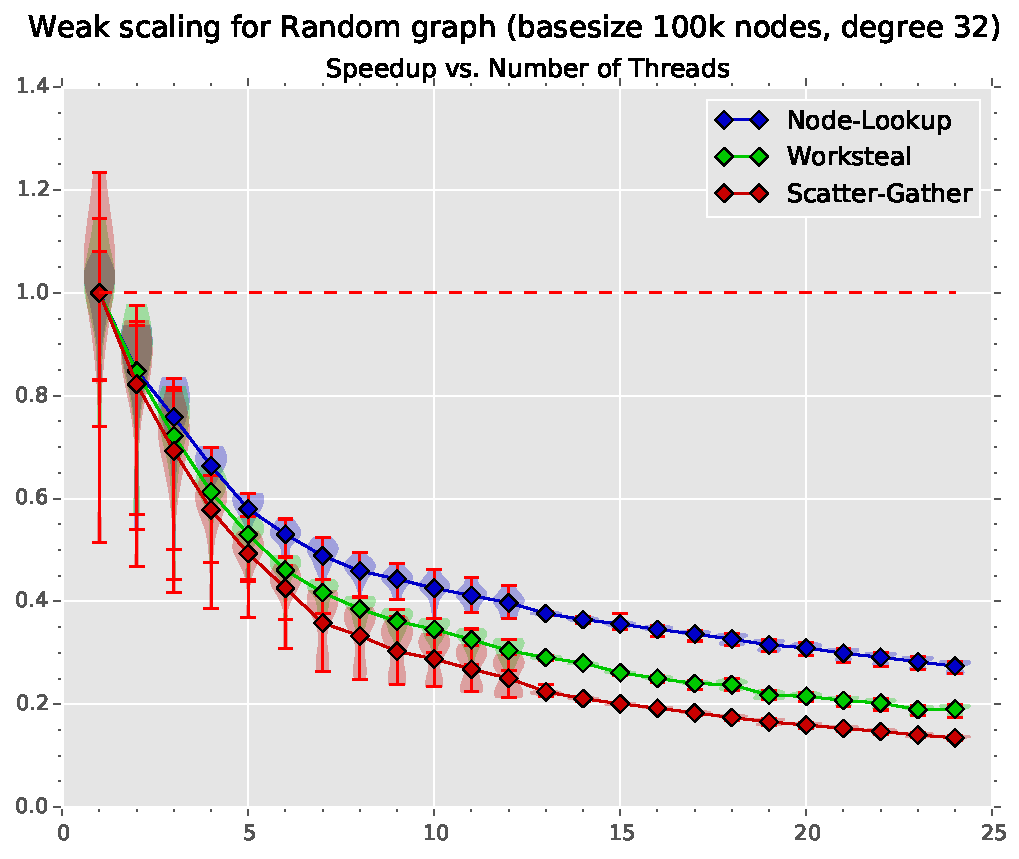
\includegraphics[width=\columnwidth]{plots/weakscaling_gtRANDOMLIN32_n1000000_deg32.pdf}
	\caption{The base size of the graphs in this weak scaling plot is 100'000 nodes.
		The Node-Lookup algorithm achieves the best performance and is only roughly 3 times slower at sorting a 24Mio node graph on 24 threads than in the base case. The Worksteal implementation takes approx. 5 times longer than the base case. \\
	It can also be noted that there is a relatively high speedup drop between 12 and 13 threads.
	This can be explained by the hardware on which the program is run. In fact, there are 24 cores but only 12 of them are on the same socket.
	Also the variance of the timings almost vanishes thread numbers higher than 12.
}
	\label{fig:weakscaling}
\end{figure}
%
\begin{figure}[ht]
	\centering
	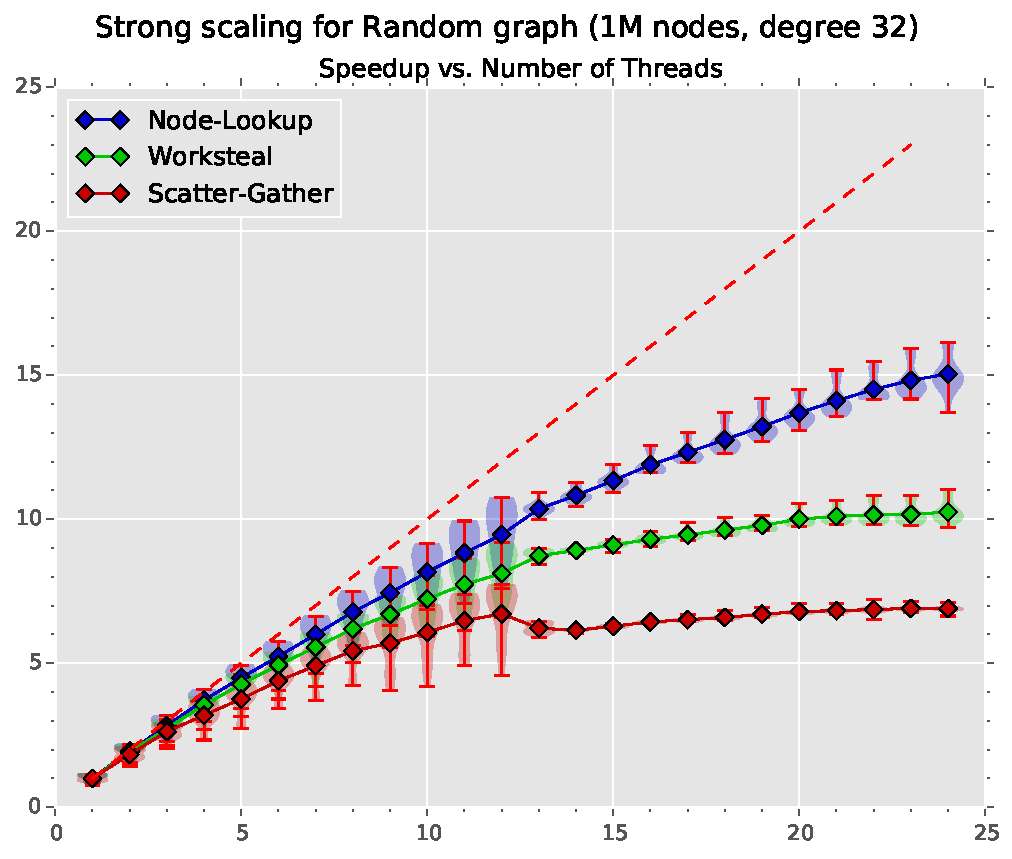
\includegraphics[width=\columnwidth]{plots/strongscaling_gtRANDOMLIN_n1000000_deg32.pdf}
	\caption{The Node-Lookup algorithm again shows better scaling than the Worksteal algorithm. On 24 cores they achieve a speedup factor of 15x and 10x respectively.}
	\label{fig:strongscaling}
\end{figure}
%
However, bearing in mind the inherently serial nature of the topological sorting algorithm, both implementations can be viewed as very successful parallelizations as compared to the simple Scatter-Gather approach.



%%%%%%%%%%%%%%%%%%%%%%%%%%%%%%%%%%%%%%%%%%%%%%%%%%%%%%%%%%%%%%%%%
% GRAPH TYPES
%%%%%%%%%%%%%%%%%%%%%%%%%%%%%%%%%%%%%%%%%%%%%%%%%%%%%%%%%%%%%%%%%
\mypar{Dependency on Graph Type} So far, our analysis only considered a sparse random graph of average node degree 32.
Next, we want to look at the performance of parallel topological sorting applied to other graph types.
All the graphs we analyzed for this purpose were sparse with the number of edges $|E|$ much smaller than the maximum possible number of vertices $|V|(|V|-1)$.
In particular, the the number of edges in the graph scales linearly with the graph size, $|E| \sim \mathcal{O} ( |V| )$). \\
It should also be noted that all of the analyzed graphs are artificial (i.e. they do not come from real-world datasets but are rather constructed to meet some requirements).
Nevertheless, the performance analysis that was carried out in this report should still be a good indicator of how the topological sorting algorithms would scale on real-world graphs with similar densities. \\
The strong scaling of the Node-Lookup algorithm for several different input graphs is presented in Figure \ref{fig:strongscaling_graphtypes}.
In fact, it clearly shows how the scaling behavior of the algorithm gets better for graphs with higher density, i.e. more edges per node.
%
\begin{figure}[ht]
	\centering
	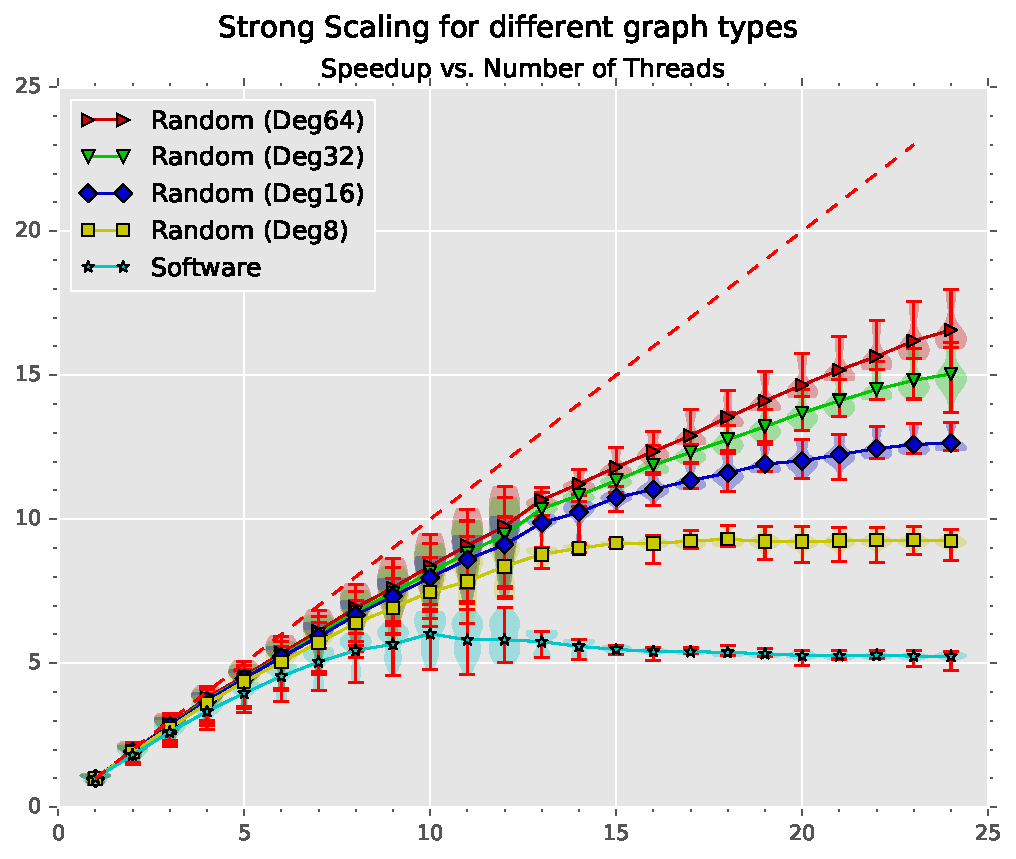
\includegraphics[width=\columnwidth]{plots/strongscaling_gtALL_n1000000.pdf}
	\caption{Strong scaling of the Node-Lookup algorithm for several different input graphs of size 1Mio nodes. The scaling is better for random graphs with higher node degree than for those with low node degree.
		The software graph (average node degree approx. 2) achieves a speedup of roughly 6x on 10 threads but does not scale any further.
}
	\label{fig:strongscaling_graphtypes}
\end{figure}
%
The software graph was constructed according to the description in \cite{musco2014generative} and should to some extend be a realistic emulation of a real world software graph. \\
The average node degree in such a software graph is very low meaning that the overhead required to synchronize the threads becomes large compared to the work that needs to be performed which in turn destroys most of the parallelism. \\
%
While similar results can be expected for real-world graphs with similar densities, the performance of the algorithms on such graphs was not tested yet and an investigation of such could be content of further research.
